\documentclass[12pt]{extarticle}

\usepackage{amsmath}
\usepackage{unicode-math}
\usepackage{xltxtra}
\usepackage{xgreek}

\setmainfont{Liberation Serif}

\usepackage{tabularx}

\pagestyle{empty}

\usepackage{geometry}
\geometry{a4paper, total={190mm,275mm}, left=10mm, top=10mm}

\usepackage{graphicx}
\graphicspath{ {images/} }

\usepackage{wrapfig}

\begin{document}

\begin{table}
    \small
    \begin{tabularx}{\textwidth}{ c X r }
        \begin{tabular}{ c }
            
\includegraphics[scale=0.4]{ελληνική}         \\
            ΕΛΛΗΝΙΚΗ ΔΗΜΟΚΡΑΤΙΑ                           \\
            ΥΠΟΥΡΓΕΙΟ ΠΑΙΔΕΙΑΣ \& ΘΡΗΣΚΕΥΜΑΤΩΝ            \\
            ΠΕΡΙΦΕΡΕΙΑΚΗ Δ/ΝΣΗ Α/ΘΜΙΑΣ \& Β/ΘΜΙΑΣ ΕΚΠ/ΣΗΣ \\
            ΚΕΝΤΡΙΚΗΣ ΜΑΚΕΔΟΝΙΑΣ                          \\
            Δ/ΝΣΗ Β/ΘΜΙΑΣ ΕΚΠ/ΣΗΣ ΑΝ. ΘΕΣ/ΝΙΚΗΣ           \\
            10ο ΓΕΝΙΚΟ ΛΥΚΕΙΟ ΘΕΣ/ΝΙΚΗΣ
        \end{tabular}
         &  &
        \begin{tabular}{ r }
            Σχολικό Έτος: 2022 - 2023     \\
            Εξ. Περίοδος: Μαΐου - Ιουνίου \\
            Μάθημα: Γεωμετρία Β Λυκείου   \\
            Εισηγητής: Λόλας              \\ \\
            Θεσσαλονίκη, 26 / 05 / 2023
        \end{tabular}
    \end{tabularx}
\end{table}

\part*{\centering{Θέματα}}
\section*{Θέμα 1}
\noindent

\begin{enumerate}
    \item[α)] Να αποδείξετε ότι αν $Α$ ένα ενδεχόμενο ενός δειγματοχώρου και $Α'$ το συμπλήρωμά του, τότε
        $$P(Α')=1-P(Α)$$.
        \hspace*{\fill} \textbf{Μονάδες 10}

    \item[β)] Να χαρακτηρίσετε τις παρακάτω προτάσεις με Σωστό ή Λάθος
        \begin{enumerate}
            \item [i.] Το τετράγωνο της κάθετης πλευράς ενός ορθογωνίου τριγώνου ισούται με το γινόμενο της κάθετης πλευράς με την υποτείνουσα.
            \item [ii.] Το μήκος ενός τόξου $α$ ακτινίων σε κύκλο ακτίνας $R$ είναι $l=αR$.
            \item [iii.] Ο λόγος ομοιότητας των εμβαδών δύο όμοιων σχημάτων ισούται με τον λόγο ομοιότητας των πλευρών του.
            \item [iv.] Κανονικό πολύγωνο είναι το σχήμα που έχει όλες τις πλευρές του ίσες.
            \item [v.] Σε τρίγωνο με πλευρές $α$, $β$, $γ$, αν ισχύει $β^2<α^2+γ^2$ τότε $\hat{Β}<90^{\circ}$.\hspace*{\fill}\textbf{Μονάδες 10}
        \end{enumerate}
\end{enumerate}

\section*{Θέμα 2 ()}
\noindent
\begin{enumerate}
    \item[α)]  \hspace*{\fill} \textbf{Μονάδες 9}
    \item[β)]   \hspace*{\fill} \textbf{Μονάδες 4}
    \item[γ)]  \hspace*{\fill} \textbf{Μονάδες 3}
    \item[δ)]  \hspace*{\fill} \textbf{Μονάδες 9}
\end{enumerate}

\section*{Θέμα 3}

\noindent

\begin{wrapfigure}[3]{r}{0.38\textwidth}
    \centering
    \vspace{-50pt}
    \hspace{-80pt}
    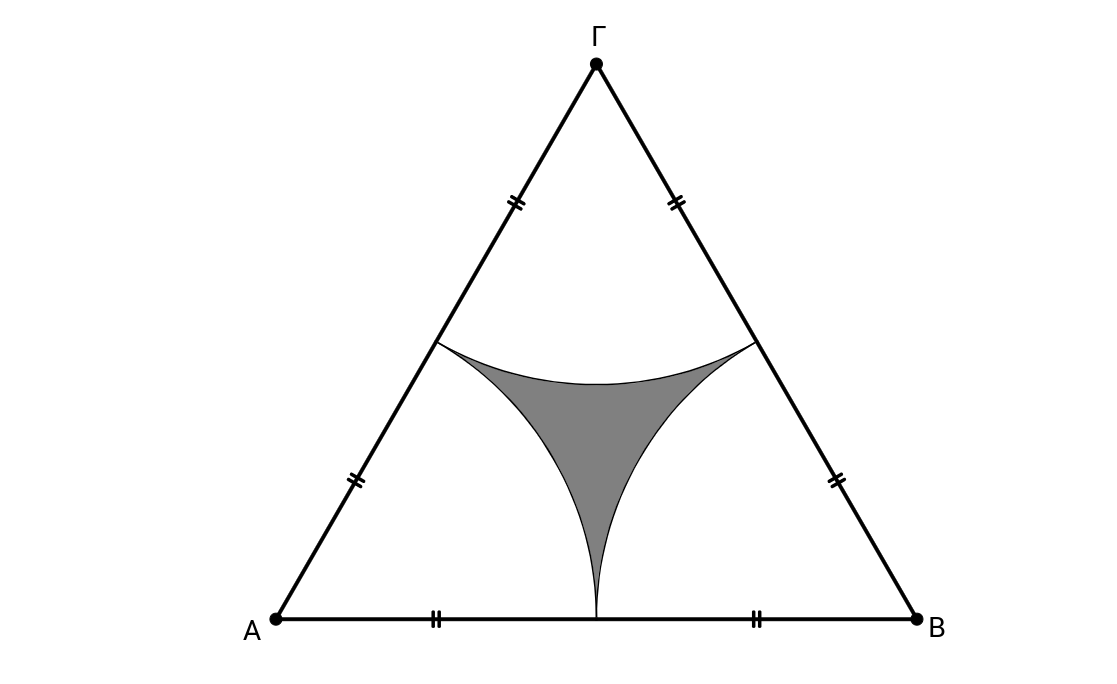
\includegraphics[width=0.38\textwidth]{2017BGeo3}
\end{wrapfigure}

Έστω ισόπλευρο τρίγωνο πλευράς $2R$. Με κέντρο κάθε κορυφή εγγράφουμε στο τρίγωνο κυκλικούς τομείς ακτίνας $R$ όπως το διπλανό σχήμα.
\begin{enumerate}
    \item[α)] Να βρείτε την περίμετρο του γραμμοσκιασμένου σχήματος. \hspace*{\fill} \textbf{Μονάδες 9}
    \item[β)]  Να δείξετε ότι το ύψος του τριγώνου είναι $R\sqrt{3}$. \hspace*{\fill} \textbf{Μονάδες 4}
    \item[γ)]  Να δείξετε ότι το εμβαδό του τριγώνου είναι $R^2\sqrt{3}$. \hspace*{\fill} \textbf{Μονάδες 3}
    \item[δ)]  Να υπολογίσετε το εμβαδό του γραμμοσκιασμένου τμήματος. \hspace*{\fill} \textbf{Μονάδες 9}
\end{enumerate}

\section*{Θέμα 4 ()}
\noindent


\begin{enumerate}
    \item[α)]  \hspace*{\fill} \textbf{Μονάδες 9}
    \item[β)]   \hspace*{\fill} \textbf{Μονάδες 4}
    \item[γ)]  \hspace*{\fill} \textbf{Μονάδες 3}
    \item[δ)]  \hspace*{\fill} \textbf{Μονάδες 9}
\end{enumerate}

\begin{table}[htb]
    \begin{tabularx}{\textwidth}{ X c X c X}
         &
        \begin{tabular}[t]{ c }
            Ο Δ/ντης \\ \\ \\ \\
            Παπαδημητρίου Χρήστος
        \end{tabular}
         &   &
        \begin{tabular}[t]{ c }
            Ο εισηγητής \\ \\ \\ \\
            Λόλας Κωνσταντίνος
        \end{tabular}
         &
    \end{tabularx}
\end{table}
\end{document}